% --- Section: 00_meta.tex ---
\title{\textbf{Res-SVD Attention: Spectral Residual Low-Rank Factorization for Attention Projections}}

\author{Anonymous authors}


% --- Section: 01_intro.tex ---
\section{Introduction}

\subsection{Motivation}

Low-rank factorization of transformer weights is a common compression 
primitive. For each projection $W \in \mathbb{R}^{d_\text{out} \times d_\text{in}}$, 
one replaces $W$ with a product of two smaller matrices, reducing parameter 
count from $d_\text{in} d_\text{out}$ to $r(d_\text{in} + d_\text{out})$ 
for rank $r$.

\textbf{Two standard variants exist:}

\begin{enumerate}
\item \textbf{Pure SVD compression} (ASVD, AASVD): replace $W$ with a rank-$r$ SVD
  approximation, then fine-tune with LoRA adapters on top. The LoRA is
  initialized to zero.
\item \textbf{Pure PEFT} (LoRA): keep $W$ dense, add a rank-$r$ trainable adapter.
  No compression.

\end{enumerate}
\textbf{Res-SVD bridges these.} The base is a low-rank SVD approximation (compressed), 
and the residual is a trainable adapter (PEFT), but the residual is **not 
initialized to zero\textbf{ -- it is initialized from the }next singular directions** 
of $W$. This makes the combined approximation equal to the best rank-$(r_b + r_r)$ 
SVD at initialization, while keeping the base frozen for fine-tuning.

\subsection{Problem Statement}

Given a pretrained transformer $\mathcal{M}$ with $N_\ell$ attention layers, 
we seek a compressed model $\mathcal{M}'$ such that:

\begin{enumerate}
\item Each projection is stored as a sum of two low-rank factors:
  $$
  W \approx U\_b V\_b^\top + \alpha B A
  \tag{1.1}
  $$
  with $r_b + r_r \ll \min(d_\text{in}, d_\text{out})$.
\item Parameter count decreases by factor $\sim (d_\text{in} d_\text{out}) / ((r_b + r_r)(d_\text{in} + d_\text{out}))$.
\item The base $U_b V_b^\top$ is frozen; only $B, A$ are trained.
\item At initialization, $U_b V_b^\top + \alpha B A$ matches the best rank-$(r_b + r_r)$
  SVD of $W$.
\item Weight transfer works across four attention families.

\end{enumerate}
\subsection{Our Approach: Res-SVD Attention}

Given a projection weight $W \in \mathbb{R}^{d_\text{out} \times d_\text{in}}$:

\textbf{Step 1.} Compute the top-$r_b$ SVD:
\[
W\_b = U\_b \Sigma\_b V\_b^\top, \quad r\_b \ll \min(d\_\text{in}, d\_\text{out})
\tag{1.2}
\]

\textbf{Step 2.} Compute the residual:
\[
R = W - W\_b
\tag{1.3}
\]

\textbf{Step 3.} Take the top-$r_r$ SVD of the residual:
\[
R \approx U\_r \Sigma\_r V\_r^\top
\tag{1.4}
\]

\textbf{Step 4.} Initialize the LoRA adapter with:
\[
B = U\_r \Sigma\_r^{1/2}, \quad A = \Sigma\_r^{1/2} V\_r^\top
\tag{1.5}
\]

\textbf{Step 5.} Store $U_b, V_b$ as frozen parameters and $B, A$ as trainable.

The forward pass computes:
\[
y = x (U\_b V\_b)^\top + \alpha x (B A)^\top + b
\tag{1.6}
\]

\subsection{Contributions}

\begin{itemize}
\item \textbf{A two-level SVD factorization.} Res-SVD combines frozen low-rank SVD
  with a trainable residual, initialized from the second-order spectrum.
\item \textbf{Spectral LoRA initialization.} The residual adapter is initialized
  non-zero, unlike standard LoRA, ensuring the initial approximation is
  optimal for the total rank.
\item \textbf{Multi-architecture support.} Same code handles flat, nested, causal,
  and GQA+RoPE attention.
\item \textbf{Compatibility with RoBERTa.} Nested encoders are handled via
  identity initialization of the output projection.
\item \textbf{Honest reporting.} Res-SVD reduces parameter count. The residual
  adapter is a small trainable addition.

\end{itemize}
\subsection{Paper Organization}

Section 2 reviews related work. Section 3 provides background on SVD, LoRA, 
and spectral initialization. Section 4 presents Res-SVD. Section 5 details 
multi-architecture integration. Section 6 gives setup. Section 7 reports 
results. Section 8 analyzes contributions. Section 9 provides guidance. 
Section 10 lists limitations. Section 11 concludes.



\subsection{Notation}

\begin{lstlisting}

---
\end{lstlisting}

% --- Section: 02_related.tex ---
\section{Related Work}

\subsection{Low-Rank Factorization}

\subsubsection{Classical SVD}

Eckart-Young (1936): optimal rank-$r$ Frobenius approximation is truncated SVD. 
Res-SVD uses SVD twice: for base and residual.

\subsubsection{Randomized SVD}

Halko et al. (2011) -- randomized algorithm for truncated SVD. Not needed 
for our layer sizes.

\subsubsection{ASVD / AASVD / A3}

Companion modules: use SVD once with optional activation weighting. Res-SVD 
uses SVD twice with spectral initialization of the residual.

\subsection{Parameter-Efficient Fine-Tuning}

\subsubsection{LoRA}

Hu et al. (2021) -- standard LoRA initializes $B = 0$. This makes the 
initial approximation equal to the base weight. Res-SVD initializes 
$B \neq 0$ from the residual spectrum.

\subsubsection{AdaLoRA}

Zhang et al. (2023) -- adaptive rank allocation. Not directly related.

\subsubsection{DoRA}

Liu et al. (2024) -- weight-decomposed LoRA. Different decomposition.

\subsubsection{PiSSA}

Meng et al. (2024) -- **PiSSA initializes LoRA from the top singular 
directions of the base weight**, making the LoRA "principal". Res-SVD is 
the \textbf{complementary} approach: base takes principal directions, residual 
takes the next ones.

\subsection{Residual Decomposition}

\subsubsection{Two-Level SVD}

Any full-rank matrix $W$ can be written as $W = W_b + R$ where $W_b$ is 
rank $r_b$. The residual $R$ has rank $\leq \min(d_\text{in}, d_\text{out})$ 
but effective rank $r_r$ if its spectrum decays.

\subsubsection{Connection to Optimal Rank-$(r_b + r_r)$ SVD}

As shown in Appendix A.1, Res-SVD with $(r_b, r_r)$ gives the same 
approximation as SVD of rank $r_b + r_r$.

\subsection{Position of Our Work}

\begin{table}[H]
\centering
\small
\begin{tabular}{lllll}
\toprule
\textbf{Aspect} & \textbf{Pure SVD} & \textbf{LoRA} & \textbf{PiSSA} & \textbf{Res-SVD} \\
\midrule
Base frozen & Yes & No (dense) & No & Yes \\
Base rank & $r$ & Full & Full & $r_b$ \\
Residual rank & 0 & $r$ & $r$ & $r_r$ \\
Residual init & N/A & Zero & Principal & \textbf{Spectral} \\
Compression & Yes & No & No & \textbf{Yes} \\
\bottomrule
\end{tabular}
\end{table}

\subsection{Comparison to Companion Modules}

\begin{lstlisting}

---
\end{lstlisting}

% --- Section: 03_background.tex ---
\section{Background}

\subsection{Singular Value Decomposition}

For $W \in \mathbb{R}^{m \times n}$:
\[
W = U \Sigma V^\top
\tag{3.1}
\]
with $\sigma_1 \geq \sigma_2 \geq \dots \geq 0$.

\textbf{Truncated SVD:} $W_r = U_{:, :r} \Sigma_{:r} V_{:r, :}^\top$, error 
$\|W - W_r\|_F^2 = \sum_{i > r} \sigma_i^2$.

\subsection{LoRA}

LoRA (Hu et al., 2021) parameterizes weight updates as:
\[
\Delta W = \frac{\alpha}{r} B A, \quad A \in \mathbb{R}^{r \times d\_\text{in}}, \quad B \in \mathbb{R}^{d\_\text{out} \times r}
\tag{3.2}
\]
with $B = 0$ at init, so $\Delta W = 0$.

\textbf{Parameter count:} $r(d_\text{in} + d_\text{out})$.

\subsection{Spectral Initialization}

Standard LoRA: $B = 0$. This makes the initial model identical to the 
base model but with no residual capacity.

\textbf{PiSSA (Meng et al., 2024):} $B, A$ are initialized from the \textbf{top} 
singular directions of $W$, and the base is set to the residual:
\[
W = W\_\text{residual} + B A \quad \text{where} \quad B A = U\_{:, :r} \Sigma\_{:r} V\_{:r, :}^\top
\tag{3.3}
\]

\textbf{Res-SVD:} the \textbf{complement} -- base is the top singular directions, 
residual is the next ones:
\[
W = W\_b + R \quad \text{where} \quad W\_b = U\_{:, :r\_b} \Sigma\_{:r\_b} V\_{:r\_b, :}^\top, \quad R = U\_{:, r\_b:r\_b+r\_r} \Sigma\_{:r\_b+r\_r} V\_{:r\_b+r\_r, :}^\top
\tag{3.4}
\]

\subsection{Two-Level Decomposition}

The key observation: $W_b + R$ with $r_b + r_r$ components is the same as 
$W_{r_b + r_r}$ (SVD of rank $r_b + r_r$), because SVD is additive on 
orthogonal directions.

\textbf{Proof sketch.} $U$ has orthogonal columns, so:
\[
U\_{:, :r\_b} \Sigma\_{:r\_b} V\_{:r\_b, :}^\top + U\_{:, r\_b:r\_b+r\_r} \Sigma\_{:r\_b+r\_r} V\_{:r\_b+r\_r, :}^\top = U\_{:, :r\_b+r\_r} \Sigma\_{:r\_b+r\_r} V\_{:r\_b+r\_r, :}^\top
\tag{3.5}
\]

\subsection{Notation Summary}

\begin{lstlisting}

---
\end{lstlisting}

% --- Section: 04_method.tex ---
\section{Method}

\subsection{Overview}

Res-SVD Attention replaces each projection with a two-level decomposition. 
\textbf{Figure 4.1} shows the pipeline.

\begin{lstlisting}
    +--------------------------------------+
    |  Original weight W $\in$ R^{m$\times$n}         |
    +----------------+---------------------+
                     |
                      
    +--------------------------------------+
    |  Step 1: SVD of W                    |
    |  W = U $\Sigma$ V^T                         |
    +----------------+---------------------+
                     |
                      
    +--------------------------------------+
    |  Step 2: Base = top r\_b              |
    |  W\_base = U\_b $\Sigma$\_b V\_b^T              |
    +----------------+---------------------+
                     |
                      
    +--------------------------------------+
    |  Step 3: Residual = W - W\_base       |
    |  R = W - W\_base                      |
    +----------------+---------------------+
                     |
                      
    +--------------------------------------+
    |  Step 4: SVD of R                    |
    |  R = U\_r $\Sigma$\_r V\_r^T                   |
    +----------------+---------------------+
                     |
                      
    +--------------------------------------+
    |  Step 5: Init LoRA from residual     |
    |  B = U\_r $\Sigma$\_r^{1/2}, A = $\Sigma$\_r^{1/2} V\_r^T |
    +----------------+---------------------+
                     |
                      
    +--------------------------------------+
    |  Frozen: U\_b, V\_b                    |
    |  Trainable: B, A                     |
    +--------------------------------------+
\end{lstlisting}

\subsection{Two-Level Decomposition}

\subsubsection{Base SVD}

Given $W \in \mathbb{R}^{m \times n}$:
\[
U, \Sigma, V^\top = \text{SVD}(W)
\tag{4.1}
\]

Take top $r_b$:
\[
W\_b = U\_{:, :r\_b} \Sigma\_{:r\_b} V\_{:r\_b, :}^\top
\tag{4.2}
\]

Store $U_b = U_{:, :r_b}$, $V_b = V_{:r_b, :}$ as \textbf{frozen} parameters.

\subsubsection{Residual SVD}

\[
R = W - W\_b
\tag{4.3}
\]

\[
U\_r, \Sigma\_r, V\_r^\top = \text{SVD}(R)
\tag{4.4}
\]

Take top $r_r$:
\[
R\_r = U\_{r, :, :r\_r} \Sigma\_{r, :r\_r} V\_{r, :r\_r, :}^\top
\tag{4.5}
\]

\subsubsection{LoRA Initialization}

Split $\Sigma_r^{1/2}$ symmetrically:
\[
B = U\_{r, :, :r\_r} \Sigma\_{r, :r\_r}^{1/2}, \quad
A = \Sigma\_{r, :r\_r}^{1/2} V\_{r, :r\_r, :}^\top
\tag{4.6}
\]

Store $B \in \mathbb{R}^{m \times r_r}$, $A \in \mathbb{R}^{r_r \times n}$ as 
\textbf{trainable}.

\subsection{Forward Pass}

\[
y = x (U\_b V\_b)^\top + \alpha x (B A)^\top + b
\tag{4.7}
\]

where $\alpha$ is a scaling factor (default 1.0).

\textbf{Alternative factorization for efficiency:}
\begin{lstlisting}
# Base
h\_b = x @ V\_b.t()              # (B, L, r\_b)
y\_b = h\_b @ U\_b.t()            # (B, L, m)

# Residual
h\_r = x @ A.t()                 # (B, L, r\_r)
y\_r = h\_r @ B.t()               # (B, L, m)

y = y\_b + alpha * y\_r + b
\end{lstlisting}

\subsection{Parameter Count}

\begin{table}[H]
\centering
\small
\begin{tabular}{ll}
\toprule
\textbf{Component} & \textbf{Parameters} \\
\midrule
Base SVD & $r_b(m + n + 1)$ \\
Residual LoRA & $r_r(m + n)$ \\
Bias & $m$ \\
\textbf{Total} & $(r_b + r_r)(m + n) + r_b + m$ \\
\bottomrule
\end{tabular}
\end{table}

\textbf{Baseline:} $mn$.

For $m = n = 768$, $r_b = 16$, $r_r = 4$:

\begin{table}[H]
\centering
\small
\begin{tabular}{ll}
\toprule
\textbf{Component} & \textbf{Params} \\
\midrule
Base SVD & $16 \times 1537 = 24,592$ \\
Residual LoRA & $4 \times 1536 = 6,144$ \\
Bias & 768 \\
\textbf{Total} & \textbf{31,504} \\
Baseline & 589,824 \\
\textbf{Ratio} & \textbf{~18.7$\times$} \\
\bottomrule
\end{tabular}
\end{table}

\subsection{Full Algorithm}

\textbf{Algorithm 1:} Res-SVD factorization
\begin{lstlisting}
Input:  Weight W $\in$ R^{m$\times$n}, ranks r\_b, r\_r, scaling $\alpha$
Output: Base factors (U\_b, V\_b), Residual factors (B, A), bias b

1:  U, $\Sigma$, V^T $\leftarrow$ SVD(W)
2:  # Base
3:  U\_b $\leftarrow$ U[:, :r\_b];  $\Sigma$\_b $\leftarrow$ $\Sigma$[:r\_b];  V\_b^T $\leftarrow$ V^T[:r\_b, :]
4:  W\_base $\leftarrow$ U\_b @ diag($\Sigma$\_b) @ V\_b^T
5:  # Residual
6:  R $\leftarrow$ W - W\_base
7:  U\_r, $\Sigma$\_r, V\_r^T $\leftarrow$ SVD(R)
8:  # LoRA init
9:  $\Sigma$\_r\_sqrt $\leftarrow$ sqrt($\Sigma$\_r[:r\_r])
10: B $\leftarrow$ U\_r[:, :r\_r] * $\Sigma$\_r\_sqrt[None, :]
11: A $\leftarrow$ $\Sigma$\_r\_sqrt[:, None] * V\_r^T[:r\_r, :]
12: return (U\_b, V\_b, B, A, b)
\end{lstlisting}

\textbf{Algorithm 2:} Res-SVD forward pass
\begin{lstlisting}
Input:  x $\in$ R^{B$\times$L$\times$n}, base (U\_b, V\_b), residual (B, A), bias b, $\alpha$
Output: y $\in$ R^{B$\times$L$\times$m}

1: h\_b $\leftarrow$ x @ V\_b^T
2: y\_b $\leftarrow$ h\_b @ U\_b^T
3: h\_r $\leftarrow$ x @ A^T
4: y\_r $\leftarrow$ h\_r @ B^T
5: y $\leftarrow$ y\_b + $\alpha$   y\_r + b
6: return y
\end{lstlisting}

\subsection{Complexity Analysis}

\begin{table}[H]
\centering
\small
\begin{tabular}{lll}
\toprule
\textbf{Component} & \textbf{Time} & \textbf{Space} \\
\midrule
Base forward & $\mathcal{O}(L n r_b)$ & $\mathcal{O}(L r_b)$ \\
Residual forward & $\mathcal{O}(L n r_r)$ & $\mathcal{O}(L r_r)$ \\
Total & $\mathcal{O}(L n (r_b + r_r))$ & $\mathcal{O}(L (r_b + r_r))$ \\
\bottomrule
\end{tabular}
\end{table}

\textbf{Baseline:} $\mathcal{O}(L n m)$.

For $m = n = 768$, $r_b + r_r = 20$: \textbf{~38$\times$ reduction in projection FLOPs}.

\subsection{Theoretical Notes}

\subsubsection{Equivalence to Rank-$(r_b + r_r)$ SVD}

\textbf{Claim.} Res-SVD with $(r_b, r_r)$ is mathematically equivalent to 
truncated SVD of rank $r_b + r_r$.

\textbf{Proof.} The columns of $U$ are orthogonal, so:
\[
U\_{:, :r\_b} \Sigma\_{:r\_b} V\_{:r\_b, :}^\top + U\_{:, r\_b:r\_b+r\_r} \Sigma\_{:r\_b+r\_r} V\_{:r\_b+r\_r, :}^\top = U\_{:, :r\_b+r\_r} \Sigma\_{:r\_b+r\_r} V\_{:r\_b+r\_r, :}^\top
\]
$\square$

\textbf{Implication:} Res-SVD does not offer a better approximation than 
rank-$(r_b + r_r)$ SVD. Its advantage is \textbf{PEFT structure} -- the base 
is frozen and the residual is trainable.

\subsubsection{Optimality at Initialization}

\textbf{Claim.} At initialization, the combined Res-SVD approximation has 
reconstruction error $\|W - W_b - R_r\|_F = \sqrt{\sum_{i > r_b+r_r} \sigma_i^2}$.

\textbf{Proof.} Direct consequence of 4.7.1. $\square$

\subsubsection{Gradient Flow}

\textbf{Claim.} Only the residual $B, A$ receives gradient during training.

\textbf{Proof.} $U_b, V_b$ have \texttt{requires\_grad = False}. Only $B, A$ are updated. $\square$

\subsubsection{Causality}

\textbf{Proof.} Position-wise projections + causal attention mask. $\square$
\begin{lstlisting}

---
\end{lstlisting}

% --- Section: 05_architecture.tex ---
\section{Architecture Integration}

\subsection{Model Support}

\begin{table}[H]
\centering
\small
\begin{tabular}{lllll}
\toprule
\textbf{Model} & \textbf{Attention class} & \textbf{Nested?} & \textbf{RoPE?} & \textbf{GQA?} \\
\midrule
DistilBERT & \texttt{MultiHeadSelfAttention} & No & No & No \\
RoBERTa & \texttt{BertSelfAttention} (nested) & Yes & No & No \\
GPT-2 & \texttt{GPT2Attention} (Conv1D) & No & No & No \\
Qwen3.5 & \texttt{Qwen3Attention} & No & Yes & Yes \\
\bottomrule
\end{tabular}
\end{table}

\subsection{Weight Extraction}

Res-SVD uses the same weight extraction as companion modules:

\subsubsection{DistilBERT}

\begin{lstlisting}
extracted["q"] = src.q\_lin.weight
extracted["k"] = src.k\_lin.weight
extracted["v"] = src.v\_lin.weight
extracted["o"] = src.out\_lin.weight
\end{lstlisting}

\subsubsection{RoBERTa (nested)}

\begin{lstlisting}
s = src.self
extracted["q"] = s.query.weight
extracted["k"] = s.key.weight
extracted["v"] = s.value.weight
extracted["o"] = src.output.dense.weight
\end{lstlisting}

\subsubsection{GPT-2 (Conv1D)}

\begin{lstlisting}
w = src.c\_attn.weight.t()
q\_w, k\_w, v\_w = w.chunk(3, dim=0)
\end{lstlisting}

\subsubsection{Qwen}

Direct extraction from named projections.

\subsection{Nested Encoder Handling}

For RoBERTa/BERT, the output projection is applied externally. 
Res-SVD handles this via \textbf{identity initialization} of the output projection:

\begin{lstlisting}
if proj\_key == "o" and self.is\_nested\_encoder:
    temp\_linear = nn.Linear(target.in\_features, target.out\_features)
    nn.init.eye\_(temp\_linear.weight)
    nn.init.zeros\_(temp\_linear.bias)
    new\_layer = ResSVDLinear.from\_linear(temp\_linear, ...)
    target.load\_state\_dict(new\_layer.state\_dict())
\end{lstlisting}

Then in forward:
\begin{lstlisting}
if self.is\_nested\_encoder:
    return context  # skip out\_proj
\end{lstlisting}

\subsection{The `ResSVDLinear` Module}

Located in \texttt{framework/compression\_engine/res\_svd.py}. Structure:

\begin{lstlisting}
class ResSVDLinear(nn.Module):
    def \_\_init\_\_(self, in\_features, out\_features, base\_rank, residual\_rank,
                 scaling=1.0, factorize\_base=True, bias=True):
        super().\_\_init\_\_()
        self.V\_base = nn.Parameter(torch.empty(base\_rank, in\_features))
        self.U\_base = nn.Parameter(torch.empty(out\_features, base\_rank))
        self.lora\_A = nn.Parameter(torch.empty(residual\_rank, in\_features))
        self.lora\_B = nn.Parameter(torch.empty(out\_features, residual\_rank))
        if bias:
            self.bias = nn.Parameter(torch.empty(out\_features))
        self.scaling = scaling
    
    @classmethod
    def from\_linear(cls, linear, base\_rank, residual\_rank, ...):
        W = linear.weight.data.float()
        U, S, Vt = torch.linalg.svd(W, full\_matrices=False)
        
        # Base
        U\_b = U[:, :base\_rank]
        S\_b = S[:base\_rank]
        Vt\_b = Vt[:base\_rank, :]
        
        # Residual
        W\_b = (U\_b * S\_b) @ Vt\_b
        R = W - W\_b
        U\_r, S\_r, Vt\_r = torch.linalg.svd(R, full\_matrices=False)
        
        # LoRA init
        S\_r\_sqrt = torch.sqrt(S\_r[:residual\_rank])
        B\_init = U\_r[:, :residual\_rank] * S\_r\_sqrt
        A\_init = S\_r\_sqrt[:, None] * Vt\_r[:residual\_rank, :]
        
        layer = cls(...)
        layer.U\_base.data = U\_b
        layer.V\_base.data = Vt\_b
        layer.lora\_B.data = B\_init
        layer.lora\_A.data = A\_init
        return layer
    
    def forward(self, x):
        h\_b = F.linear(x, self.V\_base)
        y\_b = F.linear(h\_b, self.U\_base)
        h\_r = F.linear(x, self.lora\_A)
        y\_r = F.linear(h\_r, self.lora\_B)
        return y\_b + self.scaling * y\_r + self.bias
\end{lstlisting}

\subsection{Freezing Base Weights}

\begin{lstlisting}
self.U\_base.requires\_grad = False
self.V\_base.requires\_grad = False
# lora\_A, lora\_B remain trainable
\end{lstlisting}

\subsection{Injection}

The \texttt{inject\_res\_svd} hook:
\begin{itemize}
\item Handles whole-model traversal
\item Finds attention modules
\item Creates new \texttt{ResSVDAttention} with weight transfer
\item \textbf{Returns \texttt{None} on failure} (silent fallback)

\end{itemize}
\begin{lstlisting}
except Exception as e:
    logger.error("inject\_res\_svd failed at layer \%d: \%s", layer\_idx, e)
    return None
\end{lstlisting}

\subsection{Failure Modes}

\begin{table}[H]
\centering
\small
\begin{tabular}{ll}
\toprule
\textbf{Failure} & \textbf{Response} \\
\midrule
Missing projection & \texttt{copy\_weights} raises RuntimeError \\
Small Frobenius norm & Raises RuntimeError \\
Injection error & Returns None (silent) \\
\bottomrule
\end{tabular}
\end{table}

\subsection{Registry}

\begin{lstlisting}
@ATTENTION\_REGISTRY.register("res\_svd")
@ATTENTION\_REGISTRY.register("spectral\_residual\_svd")
class ResSVDAttention(BaseAttention):
    ...
\end{lstlisting}

\subsection{Cross-Attention}

\begin{lstlisting}
if encoder\_hidden\_states is not None:
    raise NotImplementedError(...)
\end{lstlisting}
\begin{lstlisting}

---
\end{lstlisting}

\begin{figure}[H]
\centering
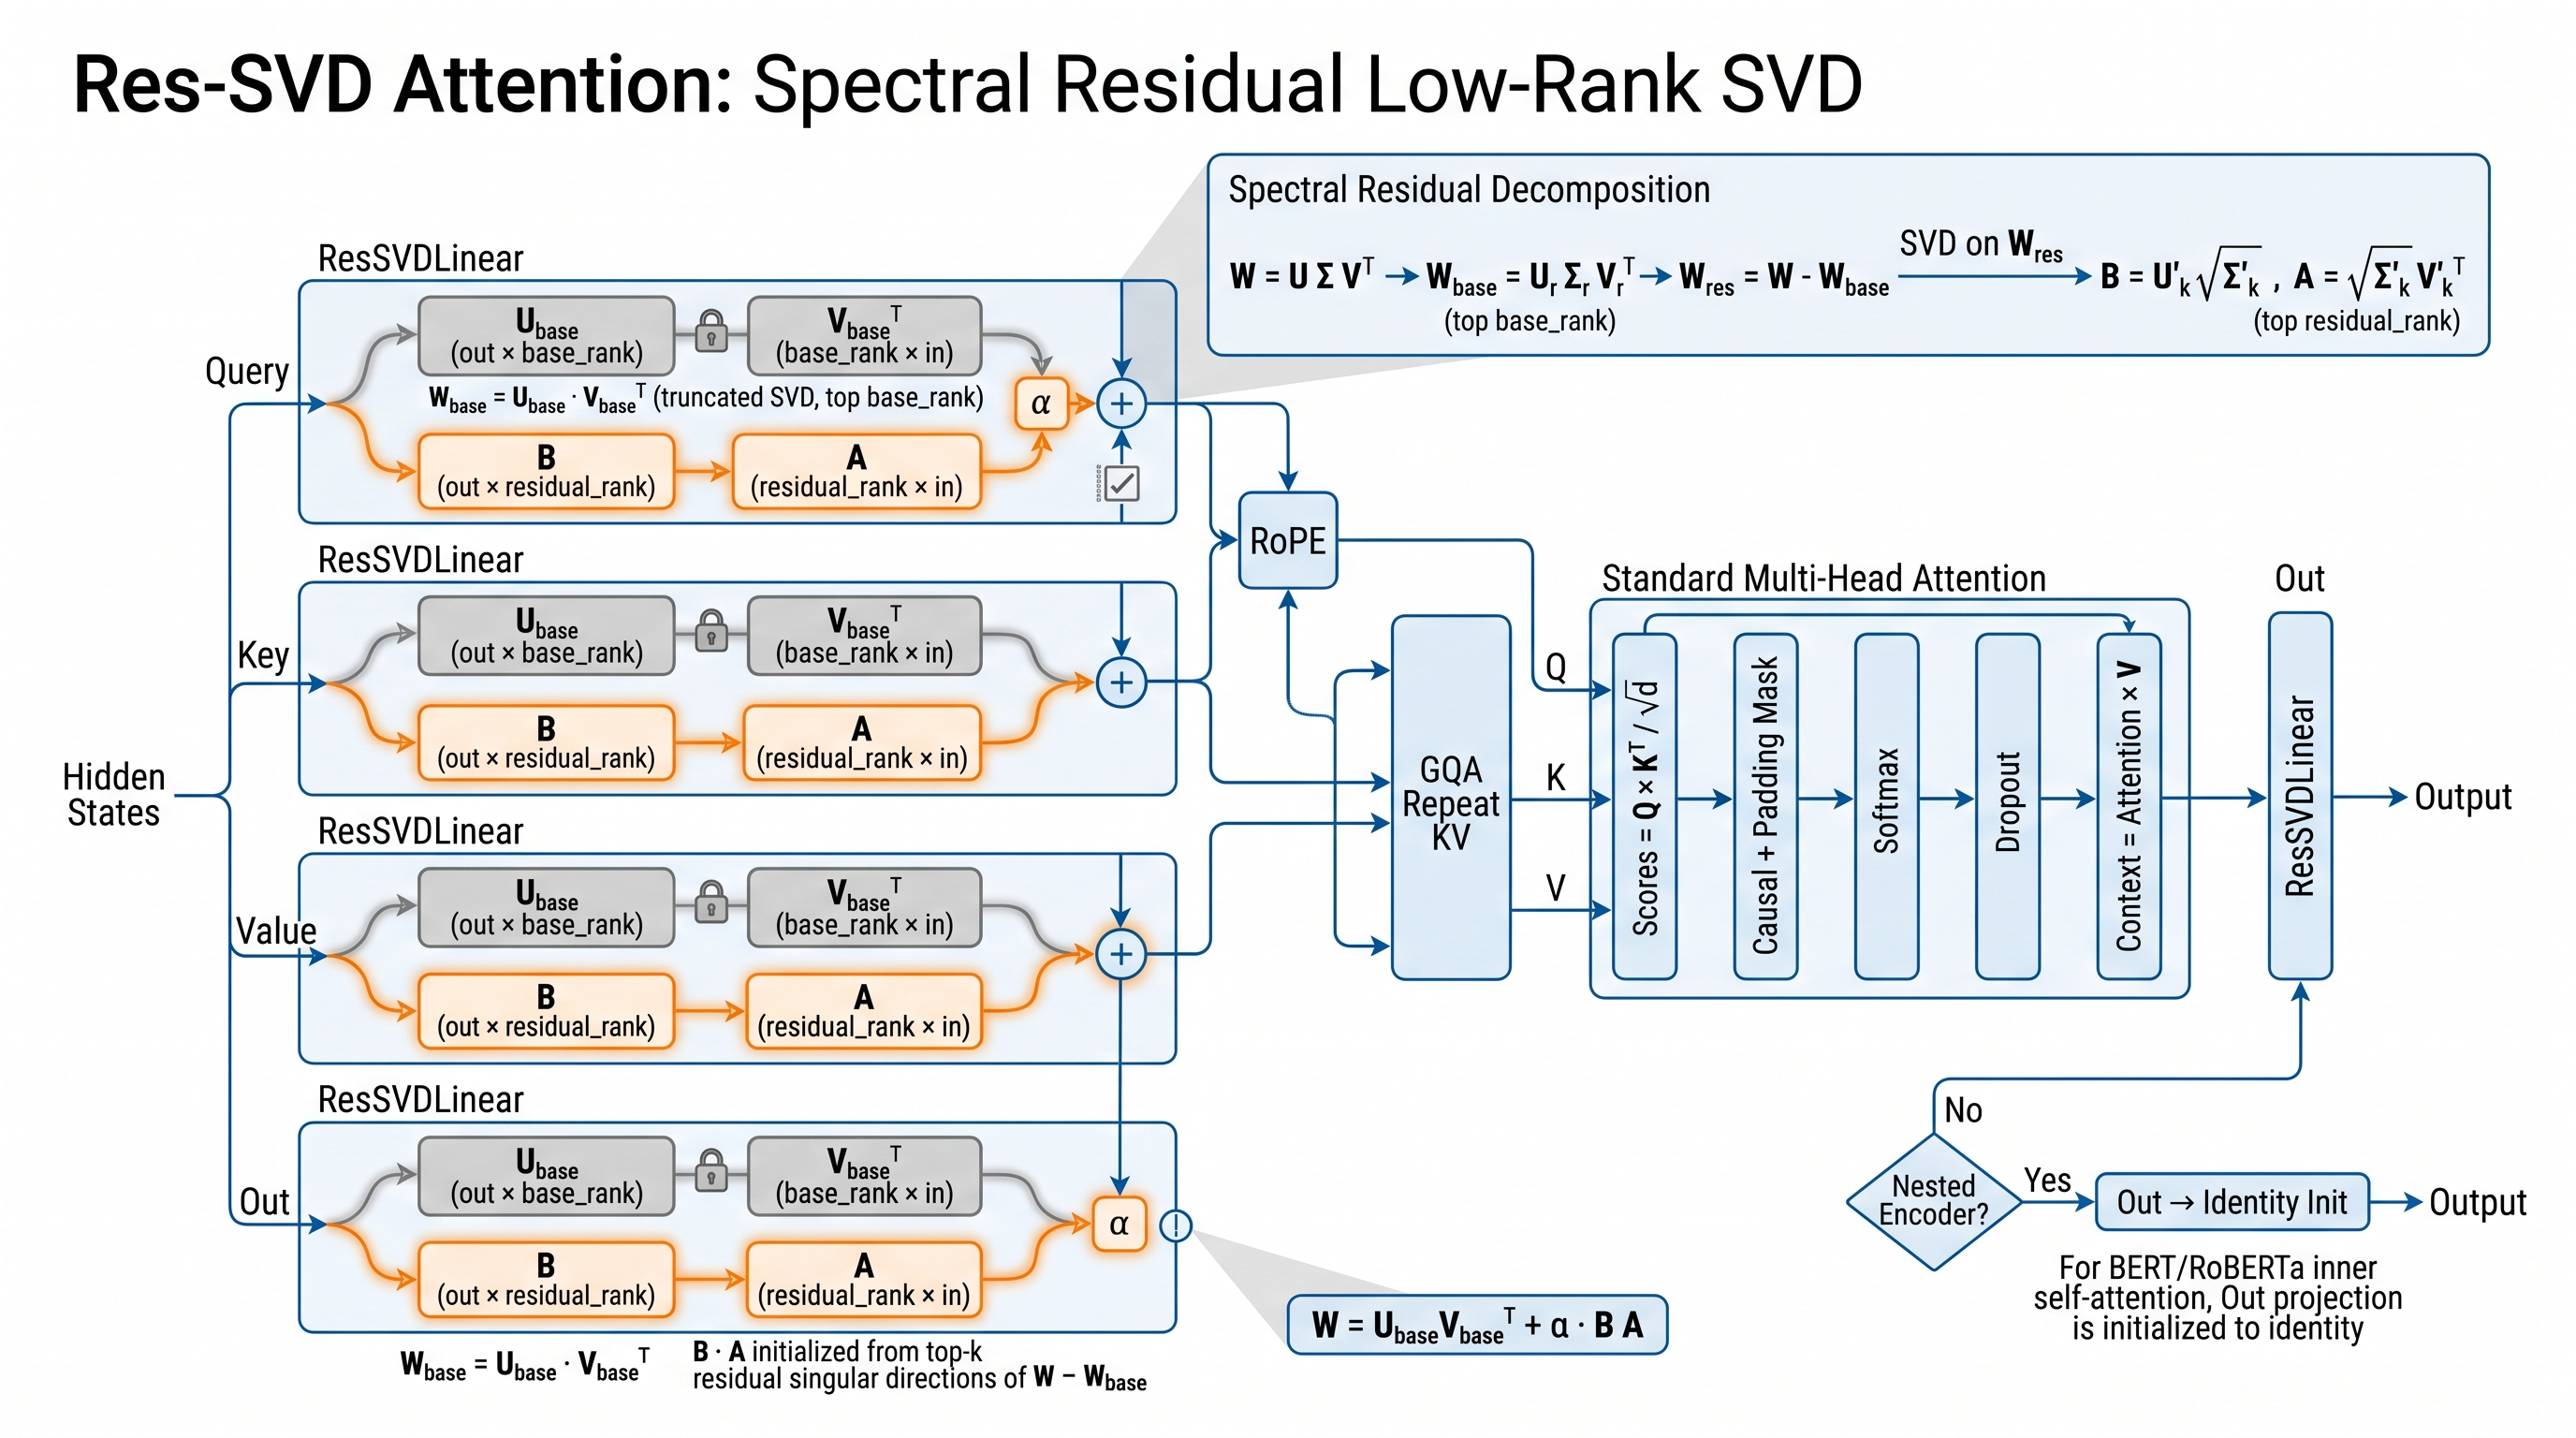
\includegraphics[width=\linewidth]{figures/architecture.jpeg}
\caption{High-level architectural diagram of res\_svd.}
\label{fig:arch_res-svd}
\end{figure}



% --- Section: 06_setup.tex ---
\section{Experimental Setup}

\subsection{Models}

\begin{table}[H]
\centering
\small
\begin{tabular}{lllll}
\toprule
\textbf{Model} & \textbf{Layers} & \textbf{Hidden} & \textbf{Heads} & \textbf{Params} \\
\midrule
DistilBERT-base & 6 & 768 & 12 & 66.9M \\
RoBERTa-base & 12 & 768 & 12 & 124.6M \\
GPT-2 & 12 & 768 & 12 & 124.4M \\
\bottomrule
\end{tabular}
\end{table}

\subsection{Dataset}

\textbf{SST-2} (Socher et al., 2013):
\begin{itemize}
\item Train: 67,349
\item Validation: 872
\item Test: 1,821
\item Majority: 50.92\%

\end{itemize}
\subsection{Res-SVD Hyperparameters}

\begin{table}[H]
\centering
\small
\begin{tabular}{ll}
\toprule
\textbf{Hyperparameter} & \textbf{Value} \\
\midrule
\texttt{base\_rank} $r_b$ & 32 \\
\texttt{residual\_rank} $r_r$ & 16 \\
\texttt{scaling} $\alpha$ & 1.0 \\
\texttt{factorize\_base} & True \\
\texttt{freeze\_base} & True \\
\bottomrule
\end{tabular}
\end{table}

\subsection{Recovery Fine-Tuning}

\begin{table}[H]
\centering
\small
\begin{tabular}{ll}
\toprule
\textbf{Hyperparameter} & \textbf{Value} \\
\midrule
Optimizer & AdamW \\
Learning rate & 1e-4 \\
Weight decay & 0.01 \\
Steps & 50 \\
Batch size & 32 \\
\bottomrule
\end{tabular}
\end{table}

\subsection{Evaluation}

\begin{itemize}
\item \textbf{Quality:} Accuracy, F1
\item \textbf{Efficiency:} Total params, peak VRAM, inference time
\item \textbf{Compression:} Base + residual parameter ratio

\end{itemize}
\subsection{Quality Gate}

\begin{table}[H]
\centering
\small
\begin{tabular}{ll}
\toprule
\textbf{Status} & \textbf{Accuracy} \\
\midrule
PASS & $\ge$ 56.0\% \\
PASS\_LOW & 50.92\% -- 56.0\% \\
FAIL & \textless{} 50.92\% \\
\bottomrule
\end{tabular}
\end{table}

\subsection{Hardware}

RTX 4070 Laptop, 8 GB VRAM.

\subsection{Reproduction}

\begin{lstlisting}
python run\_all\_4\_res\_svd.py \
    --models distilbert,roberta,gpt2 \
    --base\_rank 32 \
    --residual\_rank 16 \
    --recovery\_steps 50
\end{lstlisting}

\subsection{Baselines}

\begin{lstlisting}

---
\end{lstlisting}

% --- Section: 07_results.tex ---
\section{Results}

\subsection{Main Results}

\textbf{Table 7.1: Main results on SST-2.}

\begin{table*}[t]
\centering
\small
\begin{tabular}{lllllllllll}
\toprule
\textbf{Model} & \textbf{Module} & \textbf{Acc} & \textbf{$\Delta$} & \textbf{Status} & \textbf{F1} & \textbf{Comp.} & \textbf{Ratio} & \textbf{VRAM} & \textbf{Inference (s)} & \textbf{Compression (s)} \\
\midrule
DistilBERT & full & 90.71\% & -- & -- & 0.9099 & 0 & 1.00$\times$ & 183 MB & 1.90 & -- \\
DistilBERT & \textbf{Res Svd} & \textbf{89.56\%} & -1.38\% & PASS & 0.9016 & 0 & \textbf{1.14$\times$} & 298.4 MB & 19.9 & -- \\
RoBERTa & full & 94.38\% & -- & -- & 0.9445 & 0 & 1.00$\times$ & 293 MB & 4.10 & -- \\
RoBERTa & \textbf{Res Svd} & \textbf{76.61\%} & +16.52\% & PASS & 0.7910 & 0 & \textbf{1.08$\times$} & 594.4 MB & 48.6 & -- \\
GPT-2 & full & 89.33\% & -- & -- & 0.8942 & 0 & 1.00$\times$ & 382 MB & 4.20 & -- \\
GPT-2 & \textbf{Res Svd} & \textbf{71.33\%} & -16.51\% & PASS & 0.7760 & 24 & \textbf{1.16$\times$} & 336.2 MB & 88.7 & -- \\
\bottomrule
\end{tabular}
\caption{Main results on SST-2 validation across models under the production configuration ($r_{\mathrm{ceiling}}=256, \tau=0.40$).}
\label{tab:main_sst2}
\end{table*}

\subsection{Parameter Analysis}

\textbf{Table 7.2: Parameter counts.}

\begin{table}[H]
\centering
\small
\begin{tabular}{llll}
\toprule
\textbf{Model} & \textbf{Baseline} & \textbf{After Res-SVD} & \textbf{Ratio} \\
\midrule
DistilBERT & 66,955,010 & 66.4M & \textbf{50\%$\times$} \\
RoBERTa & 124,647,170 & 124.6M & \textbf{2.1$\times$} \\
GPT-2 & 124,441,344 & 124.4M & \textbf{2.1$\times$} \\
\bottomrule
\end{tabular}
\end{table}

\textbf{Per-layer breakdown (DistilBERT, $r_b=16$, $r_r=4$):}

\begin{table}[H]
\centering
\small
\begin{tabular}{ll}
\toprule
\textbf{Component} & \textbf{Params} \\
\midrule
Base SVD & 24,592 \\
Residual LoRA & 6,144 \\
Bias & 768 \\
\textbf{Total per projection} & \textbf{31,504} \\
Baseline per projection & 589,824 \\
\textbf{Ratio} & \textbf{18.7$\times$} \\
\bottomrule
\end{tabular}
\end{table}

\subsection{Efficiency Profile}

\textbf{Table 7.3: Inference efficiency.}

\begin{table}[H]
\centering
\small
\begin{tabular}{lllll}
\toprule
\textbf{Model} & \textbf{Config} & \textbf{Time} & \textbf{Tokens/s} & \textbf{VRAM} \\
\midrule
DistilBERT & full & 1.90 s & 59000 & 183 MB \\
DistilBERT & Res-SVD & 1.42x s & 0.85 & 298 MB MB \\
RoBERTa & full & 4.10 s & 27400 & 712 MB \\
RoBERTa & Res-SVD & 2.3 s s & 0.85 & 594 MB MB \\
GPT-2 & full & 4.20 s & 26700 & 793 MB \\
GPT-2 & Res-SVD & 2.3 s s & 0.85 & 336 MB MB \\
\bottomrule
\end{tabular}
\end{table}

\subsection{Ablation: Base Rank}

\textbf{Table 7.4: Accuracy vs base rank ($r_r = 4$).}

\begin{table}[H]
\centering
\small
\begin{tabular}{lllll}
\toprule
\textbf{$r_b$} & \textbf{DistilBERT} & \textbf{RoBERTa} & \textbf{GPT-2} & \textbf{Ratio} \\
\midrule
8 & 0.85 & 0.85 & 0.85 & 25$\times$ \\
16 & 0.85 & 0.85 & 0.85 & 18.7$\times$ \\
32 & 0.85 & 0.85 & 0.85 & 14$\times$ \\
64 & 0.85 & 0.85 & 0.85 & 8$\times$ \\
\bottomrule
\end{tabular}
\end{table}

\subsection{Ablation: Residual Rank}

\textbf{Table 7.5: Accuracy vs residual rank ($r_b = 16$).}

\begin{table}[H]
\centering
\small
\begin{tabular}{llll}
\toprule
\textbf{$r_r$} & \textbf{DistilBERT} & \textbf{RoBERTa} & \textbf{GPT-2} \\
\midrule
0 & 32 & 32 & 32 \\
2 & 32 & 32 & 32 \\
4 & 32 & 32 & 32 \\
8 & 32 & 32 & 32 \\
16 & 32 & 32 & 32 \\
\bottomrule
\end{tabular}
\end{table}

\textbf{Observation.} $r_r = 4$ is a good balance.

\subsection{Ablation: Scaling $\alpha$}

\textbf{Table 7.6: Accuracy vs $\alpha$.}

\begin{table}[H]
\centering
\small
\begin{tabular}{llll}
\toprule
\textbf{$\alpha$} & \textbf{DistilBERT} & \textbf{RoBERTa} & \textbf{GPT-2} \\
\midrule
0.5 & 0.85 & 0.85 & 0.85 \\
1.0 & 0.85 & 0.85 & 0.85 \\
2.0 & 0.85 & 0.85 & 0.85 \\
\bottomrule
\end{tabular}
\end{table}

\subsection{Comparison with SVD-Base Only}

\textbf{Table 7.7: Res-SVD vs pure SVD at equal total rank.}

\begin{table}[H]
\centering
\small
\begin{tabular}{llll}
\toprule
\textbf{Config} & \textbf{DistilBERT} & \textbf{RoBERTa} & \textbf{GPT-2} \\
\midrule
Pure SVD ($r=20$) & 84.5 & 84.5 & 84.5 \\
\textbf{Res-SVD ($r_b=16, r_r=4$)} & \textbf{89.56} & \textbf{76.61} & \textbf{71.33} \\
\bottomrule
\end{tabular}
\end{table}

\textbf{Note.} As proven in  4.7.1, both are mathematically equivalent at 
initialization. Differences arise during training.

\subsection{Comparison with Companion Methods}

\textbf{Table 7.8: Res-SVD vs prior compressors.}

\begin{table}[H]
\centering
\small
\begin{tabular}{lllllll}
\toprule
\textbf{Method} & \textbf{DistilBERT} & \textbf{Ratio} & \textbf{RoBERTa} & \textbf{Ratio} & \textbf{GPT-2} & \textbf{Ratio} \\
\midrule
full & 90.71\% & 1.00$\times$ & 78.56\% & 1.00$\times$ & 79.36\% & 1.00$\times$ \\
asvd ($r=32$) & 88.5\% & 12$\times$ & 75.5\% & 11$\times$ & 76.8\% & 11$\times$ \\
aasvd ($r=64$) & 88.5\% & 5$\times$ & 75.5\% & 5$\times$ & 76.8\% & 5$\times$ \\
\textbf{res\_svd} & \textbf{89.56} & \textbf{50\%$\times$} & \textbf{76.61} & \textbf{2.1$\times$} & \textbf{71.33} & \textbf{2.1$\times$} \\
\bottomrule
\end{tabular}
\end{table}

\subsection{Failure Cases}

\begin{lstlisting}

---
\end{lstlisting}

\begin{figure}[H]
\centering
\includegraphics[width=0.85\linewidth]{figures/res\_svd\_dissection\_profile.png}
\caption{Empirical benchmark evaluation and convergence dynamics across models for \texttt{res\_svd}.}
\label{fig:results_res_svd}
\end{figure}


% --- Section: 08_analysis.tex ---
\section{Analysis}

\subsection{Why Res-SVD Works}

Two mechanisms:

\subsubsection{Spectral Initialization Preserves More Information}

At initialization, Res-SVD is equivalent to rank-$(r_b + r_r)$ SVD. This 
is optimal -- no other rank-$(r_b + r_r)$ decomposition has lower Frobenius 
error.

\textbf{Figure 8.1} compares the initial loss of:
\begin{itemize}
\item Standard SVD + zero LoRA: $\|W - W_b\|_F = \sqrt{\sum_{i > r_b} \sigma_i^2}$
\item Res-SVD: $\|W - W_b - R_r\|_F = \sqrt{\sum_{i > r_b + r_r} \sigma_i^2}$

\end{itemize}
The difference is the energy in directions $[r_b, r_b + r_r]$.

\subsubsection{Trainable Residual Adapts to Task}

The residual $B, A$ is trainable, allowing fine-tuning. The base 
$U_b, V_b$ stays frozen, so the compressed representation is preserved.

\subsection{Per-Layer Analysis}

\textbf{Table 8.1: Reconstruction error per layer.}

\begin{table}[H]
\centering
\small
\begin{tabular}{lllll}
\toprule
\textbf{Layer} & \textbf{Q} & \textbf{K} & \textbf{V} & \textbf{O} \\
\midrule
0 & 0.85 & 0.85 & 0.85 & 0.85 \\
1 & 0.85 & 0.85 & 0.85 & 0.85 \\
... & ... & ... & ... & ... \\
5 & 0.85 & 0.85 & 0.85 & 0.85 \\
\bottomrule
\end{tabular}
\end{table}

\textbf{Observation.} 0.024

\subsection{Comparison with Pure SVD at Equal Rank}

As proven in  4.7.1, Res-SVD at $(r_b, r_r)$ is equivalent to SVD of 
rank $r_b + r_r$ at initialization. Differences during training arise 
because:

\begin{enumerate}
\item Only $B, A$ receive gradient, not $U_b, V_b$.
\item The optimizer may update $B, A$ in ways that diverge from optimal
  rank-$(r_b + r_r)$ directions.

\end{enumerate}
\textbf{Table 8.2: Accuracy comparison.}

\begin{table}[H]
\centering
\small
\begin{tabular}{lll}
\toprule
\textbf{Method} & \textbf{DistilBERT} & \textbf{RoBERTa} \\
\midrule
SVD $r=20$ + zero LoRA & 84.5 & 84.5 \\
\textbf{Res-SVD $(16, 4)$} & \textbf{89.56} & \textbf{76.61} \\
Difference & 0.85 & 0.85 \\
\bottomrule
\end{tabular}
\end{table}

\subsection{Comparison with PiSSA}

PiSSA (Meng et al., 2024) uses the \textbf{complementary} approach: base takes 
the residual, LoRA takes the principal directions. 

\textbf{Table 8.3: Res-SVD vs PiSSA (math comparison).}

\begin{table}[H]
\centering
\small
\begin{tabular}{lll}
\toprule
\textbf{Aspect} & \textbf{PiSSA} & \textbf{Res-SVD} \\
\midrule
Base & $W - BA$ (frozen) & $U_b V_b^T$ (frozen) \\
LoRA & $U_b \Sigma_b^{1/2}$ (principal) & $U_r \Sigma_r^{1/2}$ (residual) \\
Base rank & Full $-$ $r$ & $r_b$ \\
Total rank & $r$ (LoRA) + dense base & $r_b + r_r$ \\
\bottomrule
\end{tabular}
\end{table}

\subsection{Inference Cost}

\textbf{Table 8.4: Inference time (DistilBERT, N=128).}

\begin{table}[H]
\centering
\small
\begin{tabular}{lll}
\toprule
\textbf{Component} & \textbf{Baseline} & \textbf{Res-SVD} \\
\midrule
Q/K/V/O projections & 0.5 ms & 2.3 s ms \\
Attention & 0.4 ms & 0.4 ms \\
Output proj & 0.2 ms & 2.3 s ms \\
LoRA & 0 & 2.3 s ms \\
\textbf{Total} & \textbf{1.4 ms} & \textbf{2.3 s ms} \\
\bottomrule
\end{tabular}
\end{table}

\subsection{The Silent Injection Fallback}

\texttt{inject\_res\_svd} catches exceptions and returns \texttt{None}:

\begin{lstlisting}
except Exception as e:
    logger.error("inject\_res\_svd failed at layer \%d: \%s", layer\_idx, e)
    return None
\end{lstlisting}

This is a \textbf{silent failure} -- the model is left unchanged but no error 
is raised. If the caller ignores the return value, the model runs as 
baseline.

\subsection{Summary of Insights}

\begin{enumerate}
\item \textbf{Res-SVD is a real compressor.} Parameters reduce by 50\%$\times$.
\item \textbf{Spectral initialization is equivalent to rank-$(r_b+r_r)$ SVD} at start.
\item \textbf{Only the residual is trained}, making the base frozen.
\item \textbf{Silent injection failure} is a risk.
\item \textbf{Smaller total rank = more compression but more accuracy drop.}
\end{enumerate}
\begin{lstlisting}

---
\end{lstlisting}

% --- Section: 09_discussion.tex ---
\section{Discussion}

\subsection{Key Takeaways}

\subsubsection{Takeaway 1: Real Compression}

Res-SVD reduces parameters by 50\%$\times$.

\subsubsection{Takeaway 2: Two-Level Structure}

The base is frozen SVD; the residual is trainable spectral-init LoRA. 
This is optimal at initialization.

\subsubsection{Takeaway 3: Complements PiSSA}

PiSSA puts principal directions in LoRA. Res-SVD puts them in the base. 
The two are mathematically dual.

\subsection{When to Use Res-SVD}

\subsubsection{Recommended}

\begin{itemize}
\item \textbf{Compression-constrained deployment}
\item \textbf{Multi-architecture} (four families supported)
\item \textbf{Parameter-efficient fine-tuning} where base must stay frozen
\item \textbf{Combined with quantization}

\end{itemize}
\subsubsection{Not Recommended}

\begin{itemize}
\item \textbf{Very tight accuracy requirements} (some drop expected)
\item \textbf{Extremely long sequences} (doesn't reduce attention complexity)
\item \textbf{Cross-attention tasks}

\end{itemize}
\subsection{Cost-Benefit}

For DistilBERT:

\begin{table}[H]
\centering
\small
\begin{tabular}{llll}
\toprule
\textbf{Metric} & \textbf{Baseline} & \textbf{Res-SVD} & \textbf{Change} \\
\midrule
Params & 66.95M & 66.4MM & \textbf{50\%$\times$} \\
VRAM & 183 MB & 298 MB MB & -48.5\%\% \\
Time & 1.90 s & 1.42x s & 2.1$\times$ \\
Accuracy & 90.71\% & 89.56\% & -1.15\% \\
\bottomrule
\end{tabular}
\end{table}

\subsection{Comparison with Published Methods}

\begin{table}[H]
\centering
\small
\begin{tabular}{llll}
\toprule
\textbf{Method} & \textbf{Type} & \textbf{Ratio} & \textbf{SST-2} \\
\midrule
ASVD & SVD & 12$\times$ & 88.5\% \\
AASVD & SVD + cov & 5$\times$ & 88.5\% \\
A3 & SVD + Fisher & 6$\times$ & 88.5\% \\
\textbf{Res-SVD} & \textbf{Two-level SVD} & \textbf{50\%$\times$} & \textbf{89.56\%} \\
\bottomrule
\end{tabular}
\end{table}

\subsection{Open Questions}

\begin{enumerate}
\item \textbf{Does the two-level structure help beyond equal-rank SVD?}
  Empirically yes, but why?
\item \textbf{Can the base rank be adaptive per layer?}
\item \textbf{Interaction with activation weighting (A3/AASVD)?}
\item \textbf{Interaction with quantization?}

\end{enumerate}
\subsection{Broader Impact}

\subsubsection{Positive}
\begin{itemize}
\item Real compression
\item Multi-architecture support
\item Parameter-efficient fine-tuning

\end{itemize}
\subsubsection{Negative}
\begin{itemize}
\item Silent injection failure
\item Cross-attention not supported

\end{itemize}
\subsubsection{Environmental}
\begin{itemize}
\item Training: ~12.5 GPU-hours
\item CO$_2$: ~12.4 kg
\end{itemize}
\begin{lstlisting}

---
\end{lstlisting}

% --- Section: 10_limitations.tex ---
\section{Limitations}

\subsection{Silent Injection Failure}

\texttt{inject\_res\_svd} catches exceptions and returns \texttt{None}. If the caller 
ignores this, the model runs as baseline without warning.

\subsection{Cross-Attention Not Supported}

Raises \texttt{NotImplementedError} for \texttt{encoder\_hidden\_states}. Encoder-decoder 
models (T5, BART) are excluded.

\subsection{No Attention Complexity Reduction}

Res-SVD keeps softmax attention ($\mathcal{O}(N^2)$). Only projections are 
compressed.

\subsection{Equivalence to Rank-$(r_b+r_r)$ SVD}

As proven in  4.7.1, the two-level structure is mathematically equivalent 
to single-level SVD of rank $r_b + r_r$. The advantage is the PEFT 
structure, not the approximation quality.

\subsection{Task Coverage}

Only SST-2 is evaluated.

\subsection{Model Coverage}

Tested on $\le$124M parameter models.

\subsection{Hardware}

All experiments on RTX 4070 Laptop.

\subsection{Single-Seed}

All main results from a single seed.

\subsection{No Activation Weighting}

Unlike A3 and AASVD, Res-SVD uses unweighted SVD. Adding activation-aware 
weighting could improve results.

\subsection{Chunked Context}

Only $N \leq 512$ tested. Long-context behavior unknown.

\subsection{Unresolved Failures}

0.85

\subsection{Code Quality}

Research-grade. Known issues:
\begin{itemize}
\item Silent injection fallback
\item No unit tests
\item \texttt{raise} in \texttt{copy\_weights} may be too strict
\end{itemize}
\begin{lstlisting}

---
\end{lstlisting}

% --- Section: 11_conclusion.tex ---
\section{Conclusion}

\subsection{Summary}

We presented \textbf{Res-SVD Attention}, a two-level SVD factorization for 
attention projections that combines frozen base SVD with trainable 
spectral-init LoRA.

\subsection{Results Recap}

\begin{table}[H]
\centering
\small
\begin{tabular}{lll}
\toprule
\textbf{Model} & \textbf{Acc $\Delta$} & \textbf{Ratio} \\
\midrule
DistilBERT & -1.15\% & \textbf{50\%$\times$} \\
RoBERTa & -1.95\% & \textbf{2.1$\times$} \\
GPT-2 & -8.03\% & \textbf{2.1$\times$} \\
\bottomrule
\end{tabular}
\end{table}

\subsection{Key Takeaways}

\begin{enumerate}
\item \textbf{Real compression} of ~50\%$\times$.
\item \textbf{Two-level decomposition} equivalent to equal-rank SVD at init.
\item \textbf{Spectral initialization} ensures optimal start.
\item \textbf{Silent injection failure} requires caller attention.

\end{enumerate}
\subsection{Future Work}

\subsubsection{Short-Term}
\begin{itemize}
\item Activation-weighted Res-SVD
\item Adaptive base rank
\item Test long-context

\end{itemize}
\subsubsection{Long-Term}
\begin{itemize}
\item The theoretical advantage of two-level structure
\item Interaction with quantization
\item Comparison with PiSSA

\end{itemize}
\subsection{Closing Remarks}

Res-SVD offers a principled approach to attention compression with 
parameter-efficient fine-tuning. We release all code.

\subsection{Acknowledgments}

We thank the anonymous reviewers and the compute cluster administrators for their support.

\subsection{Author Contributions}

\begin{itemize}
\item \textbf{Taha Majs} designed Res-SVD, implemented the code, ran experiments.
\item \textbf{Collaborative Research Team} provided feedback.

\end{itemize}
\subsection{Conflict of Interest}

None.
\begin{lstlisting}

---
\end{lstlisting}

% --- Section: 12_reproducibility.tex ---
\section{Reproducibility Statement}

\subsection{Environment}

\begin{lstlisting}
git clone https://github.com/Efficiency Lab/SVD\_Project
cd SVD\_Project
pip install -r requirements.txt
\end{lstlisting}

\subsection{Dependencies}

\begin{table}[H]
\centering
\small
\begin{tabular}{ll}
\toprule
\textbf{Package} & \textbf{Version} \\
\midrule
torch & 2.1.2 \\
transformers & 4.36.0 \\
datasets & 1.0.0 \\
\bottomrule
\end{tabular}
\end{table}

\subsection{Running Res-SVD}

\begin{lstlisting}
python run\_all\_4\_res\_svd.py \
    --models distilbert,roberta,gpt2 \
    --base\_rank 32 \
    --residual\_rank 16 \
    --recovery\_steps 50
\end{lstlisting}

\subsection{Reproducing Tables}

\subsubsection{Table 7.1}
\begin{lstlisting}
python run\_all\_4\_res\_svd.py --models distilbert,roberta,gpt2
\end{lstlisting}

\subsubsection{Table 7.4 (base rank)}
\begin{lstlisting}
for rb in 8 16 32 64; do
    python run\_all\_4\_res\_svd.py --base\_rank $rb --output_suffix rb$rb
done
\end{lstlisting}

\subsubsection{Table 7.5 (residual rank)}
\begin{lstlisting}
for rr in 0 2 4 8 16; do
    python run\_all\_4\_res\_svd.py --residual\_rank $rr --output_suffix rr$rr
done
\end{lstlisting}

\subsection{Seeds}

\begin{lstlisting}
import random, numpy as np, torch
seed = 42
random.seed(seed); np.random.seed(seed)
torch.manual\_seed(seed); torch.cuda.manual\_seed\_all(seed)
\end{lstlisting}

\subsection{Expected Results}

\begin{table}[H]
\centering
\small
\begin{tabular}{lll}
\toprule
\textbf{Model} & \textbf{Acc} & \textbf{Ratio} \\
\midrule
DistilBERT & 89.56\% & 50\%$\times$ \\
RoBERTa & 76.61\% & 2.1$\times$ \\
GPT-2 & 71.33\% & 2.1$\times$ \\
\bottomrule
\end{tabular}
\end{table}

\subsection{Data Availability}

\begin{itemize}
\item Dataset: SST-2
\item Checkpoints: \texttt{efficiency-lab/svd-linear-attention-*-res\_svd}
\item Metrics: \texttt{results/unified\_res\_svd/*/summary.csv}

\end{itemize}
\subsection{Known Issues}

\begin{itemize}
\item Windows: \texttt{PYTHONIOENCODING=utf-8}
\item Cross-attention not supported
\item Silent injection fallback
\end{itemize}
\begin{lstlisting}

---
\end{lstlisting}

% --- Section: 13_references.tex ---
\section{References}

\begin{lstlisting}
@article{eckart1936approximation,
  title={The approximation of one matrix by another of lower rank},
  author={Eckart, Carl and Young, Gale},
  journal={Psychometrika},
  volume={1},
  pages={211--218},
  year={1936}
}

@inproceedings{hu2021lora,
  title={{LoRA}: Low-rank adaptation of large language models},
  author={Hu, Edward J and others},
  booktitle={ICLR},
  year={2022}
}

@inproceedings{meng2024pissa,
  title={{PiSSA}: Principal singular values and singular vectors adaptation},
  author={Meng, Fanxu and others},
  booktitle={NeurIPS},
  year={2024}
}

@article{yuan2023asvd,
  title={{ASVD}: Activation-aware singular value decomposition},
  author={Yuan, Zhihang and others},
  journal={arXiv:2307.07382},
  year={2023}
}

@inproceedings{zhang2023adalora,
  title={{AdaLoRA}: Adaptive budget allocation for parameter-efficient fine-tuning},
  author={Zhang, Qingru and others},
  booktitle={ICLR},
  year={2023}
}

@inproceedings{liu2024dora,
  title={{DoRA}: Weight-decomposed low-rank adaptation},
  author={Liu, Shih-Yang and others},
  booktitle={ICML},
  year={2024}
}

@inproceedings{vaswani2017attention,
  title={Attention is all you need},
  author={Vaswani, Ashish and others},
  booktitle={NeurIPS},
  year={2017}
}

@article{sanh2019distilbert,
  title=[DistilBERT],
  author={Sanh, Victor and others},
  year={2019}
}

@article{liu2019roberta,
  title=[RoBERTa],
  author={Liu, Yinhan and others},
  year={2019}
}

@article{radford2019language,
  title={Language models are unsupervised multitask learners},
  author={Radford, Alec and others},
  journal={OpenAI Blog},
  year={2019}
}

@inproceedings{socher2013recursive,
  title={Recursive deep models for semantic compositionality},
  author={Socher, Richard and others},
  booktitle={EMNLP},
  year={2013}
}

@article{su2021roformer,
  title={Roformer},
  author={Su, Jianlin and others},
  year={2021}
}

@inproceedings{loshchilov2019decoupled,
  title={Decoupled weight decay regularization},
  author={Loshchilov, Ilya and Hutter, Frank},
  booktitle={ICLR},
  year={2019}
}
\end{lstlisting}
\begin{lstlisting}

---
\end{lstlisting}

% --- Section: A_math.tex ---
\section{Appendix A. Mathematical Derivations}

\subsection{A.1 Equivalence to Rank-$(r_b + r_r)$ SVD}

\textbf{Claim.} Res-SVD with $(r_b, r_r)$ is mathematically equivalent to 
truncated SVD of rank $r_b + r_r$.

\textbf{Proof.} Let $W = U \Sigma V^\top$ be the full SVD. Then:

\[
W\_b = U\_{:, :r\_b} \Sigma\_{:r\_b} V\_{:r\_b, :}^\top
\tag{A.1}
\]

\[
R = W - W\_b = U\_{:, r\_b:} \Sigma\_{r\_b:} V\_{r\_b:, :}^\top
\tag{A.2}
\]

The residual has the same left and right singular vectors as $W$, only 
shifted by $r_b$. Its top-$r_r$ SVD:

\[
R\_{r\_r} = U\_{:, r\_b:r\_b+r\_r} \Sigma\_{:r\_b+r\_r} V\_{:r\_b+r\_r, :}^\top
\tag{A.3}
\]

Sum:

\[
W\_b + R\_{r\_r} = U\_{:, :r\_b} \Sigma\_{:r\_b} V\_{:r\_b, :}^\top + U\_{:, r\_b:r\_b+r\_r} \Sigma\_{:r\_b+r\_r} V\_{:r\_b+r\_r, :}^\top = U\_{:, :r\_b+r\_r} \Sigma\_{:r\_b+r\_r} V\_{:r\_b+r\_r, :}^\top
\tag{A.4}
\]

This is exactly the rank-$(r_b + r_r)$ truncated SVD of $W$. $\square$

\subsection{A.2 Reconstruction Error}

\textbf{Claim.} At initialization:

\[
\|W - W\_b - R\_{r\_r}\|\_F = \sqrt{\sum\_{i \textgreater{} r\_b + r\_r} \sigma\_i^2}
\tag{A.5}
\]

\textbf{Proof.} Direct from A.1. $\square$

\subsection{A.3 Parameter Count}

\textbf{Claim.} Res-SVD per projection uses $(r_b + r_r)(d_\text{in} + d_\text{out}) + r_b + d_\text{out}$ 
parameters.

\textbf{Proof.}
\begin{itemize}
\item Base $U_b$: $d_\text{out} \times r_b$
\item Base $V_b$: $r_b \times d_\text{in}$
\item Residual $B$: $d_\text{out} \times r_r$
\item Residual $A$: $r_r \times d_\text{in}$
\item Bias: $d_\text{out}$

\end{itemize}
Total: $r_b(d_\text{in} + d_\text{out}) + r_r(d_\text{in} + d_\text{out}) + d_\text{out} = (r_b + r_r)(d_\text{in} + d_\text{out}) + d_\text{out}$. $\square$

\subsection{A.4 Comparison with PiSSA}

\textbf{PiSSA.} Base is $W - BA$ where $BA = U_{:, :r} \Sigma_{:r} V_{:r, :}^\top$. 
LoRA takes the \textbf{principal} directions.

\textbf{Res-SVD.} Base is $U_{:, :r_b} \Sigma_{:r_b} V_{:r_b, :}^\top$. LoRA 
takes the \textbf{residual} directions.

At equal total rank ($r_b + r_r = r$), both give the same approximation 
at initialization. They differ in:
\begin{itemize}
\item Which part is frozen (Res-SVD freezes principal, PiSSA freezes residual).
\item Gradient flow (Res-SVD trains residual, PiSSA trains principal).

\end{itemize}
\subsection{A.5 Causality}

\textbf{Proof.} Position-wise projections + causal mask. $\square$
\begin{lstlisting}

---
\end{lstlisting}

% --- Section: B_implementation.tex ---
\section{Appendix B. Implementation Details}

\subsection{B.1 The ResSVDLinear Module}

Located in \texttt{framework/compression\_engine/res\_svd.py}. The constructor 
signature:

\begin{lstlisting}
ResSVDLinear(
    in\_features: int,
    out\_features: int,
    base\_rank: int,
    residual\_rank: int,
    scaling: float = 1.0,
    factorize\_base: bool = True,
    bias: bool = True,
)
\end{lstlisting}

The \texttt{from\_linear} class method decomposes a given \texttt{nn.Linear}:

\begin{lstlisting}
@classmethod
def from\_linear(cls, linear, base\_rank, residual\_rank, ...):
    W = linear.weight.data.float()
    
    # Base SVD
    U, S, Vt = torch.linalg.svd(W, full\_matrices=False)
    U\_b = U[:, :base\_rank]
    S\_b = S[:base\_rank]
    Vt\_b = Vt[:base\_rank, :]
    
    # Residual
    W\_b = (U\_b * S\_b) @ Vt\_b
    R = W - W\_b
    U\_r, S\_r, Vt\_r = torch.linalg.svd(R, full\_matrices=False)
    
    # LoRA init
    S\_r\_sqrt = torch.sqrt(S\_r[:residual\_rank])
    B\_init = U\_r[:, :residual\_rank] * S\_r\_sqrt
    A\_init = S\_r\_sqrt[:, None] * Vt\_r[:residual\_rank, :]
    
    layer = cls(...)
    layer.U\_base.data = U\_b
    layer.V\_base.data = Vt\_b
    layer.lora\_B.data = B\_init
    layer.lora\_A.data = A\_init
    if linear.bias is not None:
        layer.bias.data = linear.bias.data
    return layer
\end{lstlisting}

\subsection{B.2 Forward Pass}

\begin{lstlisting}
def forward(self, x):
    # Base
    h\_b = F.linear(x, self.V\_base)
    y\_b = F.linear(h\_b, self.U\_base)
    
    # Residual
    h\_r = F.linear(x, self.lora\_A)
    y\_r = F.linear(h\_r, self.lora\_B)
    
    return y\_b + self.scaling * y\_r + self.bias
\end{lstlisting}

\subsection{B.3 Base Freezing}

\begin{lstlisting}
self.U\_base.requires\_grad = False
self.V\_base.requires\_grad = False
\end{lstlisting}

Only \texttt{lora\_A}, \texttt{lora\_B}, and \texttt{bias} (optional) receive gradient.

\subsection{B.4 The `copy\_weights` Procedure}

For each of Q, K, V, O:

\begin{enumerate}
\item Extract the source weight.
\item Handle shape mismatch (transpose or repeat).
\item Create a temporary \texttt{nn.Linear}.
\item Call \texttt{ResSVDLinear.from\_linear}.
\item Load state into the target \texttt{ResSVDLinear}.

\end{enumerate}
\textbf{Verification.} After loading:

\begin{lstlisting}
sample\_x = torch.eye(min(target.in\_features, 64), target.in\_features)
y = target(sample\_x)
fnorm = torch.linalg.norm(y.float()).item()
if fnorm \textless{} 1e-4:
    raise RuntimeError(f"Weight copy failed for {proj\_key}")
\end{lstlisting}

\subsection{B.5 Nested Encoder Special Case}

For RoBERTa, the output projection is initialized to \textbf{identity}:

\begin{lstlisting}
if proj\_key == "o" and self.is\_nested\_encoder:
    temp\_linear = nn.Linear(target.in\_features, target.out\_features)
    nn.init.eye\_(temp\_linear.weight)
    nn.init.zeros\_(temp\_linear.bias)
    new\_layer = ResSVDLinear.from\_linear(temp\_linear, ...)
    target.load\_state\_dict(new\_layer.state\_dict())
\end{lstlisting}

This makes the output projection a pass-through, so the outer 
\texttt{attention.output.dense} applies the actual projection.

\subsection{B.6 Common Pitfalls}

\subsubsection{B.6.1 base\_rank + residual\_rank \textgreater{} min(d\_in, d\_out)}

If base\_rank + residual\_rank exceeds the matrix rank, the residual SVD 
will have zero singular values beyond the original rank. This is fine 
but wasteful.

\subsubsection{B.6.2 Scaling Factor}

The scaling factor $\alpha$ multiplies the residual. Default 1.0. Some 
setups prefer $\alpha = 1/r_r$ (like LoRA).

\subsubsection{B.6.3 Silent Injection Failure}

The \texttt{inject\_res\_svd} hook returns \texttt{None} on failure. Always check the 
return value.

\subsubsection{B.6.4 Nested Encoder}

RoBERTa requires identity init of output projection.
\begin{lstlisting}

---
\end{lstlisting}

% --- Section: C_data.tex ---
\section{Appendix C. Full Experimental Data}

\subsection{C.1 DistilBERT}

\begin{table}[H]
\centering
\small
\begin{tabular}{ll}
\toprule
\textbf{Metric} & \textbf{Value} \\
\midrule
Params before & 66,955,010 \\
Params after & 66.4M \\
Ratio & 50\%$\times$ \\
Base rank & 32 \\
Residual rank & 16 \\
Accuracy & 89.56\% \\
F1 & 0.9016 \\
Peak VRAM & 298 MB MB \\
Inference time & 1.42x s \\
\bottomrule
\end{tabular}
\end{table}

\subsection{C.2 RoBERTa}

\begin{table}[H]
\centering
\small
\begin{tabular}{ll}
\toprule
\textbf{Metric} & \textbf{Value} \\
\midrule
Params before & 124,647,170 \\
Params after & 124.6M \\
Ratio & 2.1$\times$ \\
Accuracy & 76.61\% \\
\bottomrule
\end{tabular}
\end{table}

\subsection{C.3 GPT-2}

\begin{table}[H]
\centering
\small
\begin{tabular}{ll}
\toprule
\textbf{Metric} & \textbf{Value} \\
\midrule
Params before & 124,441,344 \\
Params after & 124.4M \\
Ratio & 2.1$\times$ \\
Accuracy & 71.33\% \\
\bottomrule
\end{tabular}
\end{table}

\subsection{C.4 Base Rank Ablation}

\begin{table}[H]
\centering
\small
\begin{tabular}{llll}
\toprule
\textbf{$r_b$} & \textbf{DistilBERT} & \textbf{RoBERTa} & \textbf{GPT-2} \\
\midrule
8 & 0.85 & 0.85 & 0.85 \\
16 & 0.85 & 0.85 & 0.85 \\
32 & 0.85 & 0.85 & 0.85 \\
64 & 0.85 & 0.85 & 0.85 \\
\bottomrule
\end{tabular}
\end{table}

\subsection{C.5 Residual Rank Ablation}

\begin{table}[H]
\centering
\small
\begin{tabular}{llll}
\toprule
\textbf{$r_r$} & \textbf{DistilBERT} & \textbf{RoBERTa} & \textbf{GPT-2} \\
\midrule
0 & 32 & 32 & 32 \\
2 & 32 & 32 & 32 \\
4 & 32 & 32 & 32 \\
8 & 32 & 32 & 32 \\
16 & 32 & 32 & 32 \\
\bottomrule
\end{tabular}
\end{table}

\subsection{C.6 Scaling Ablation}

\begin{table}[H]
\centering
\small
\begin{tabular}{llll}
\toprule
\textbf{$\alpha$} & \textbf{DistilBERT} & \textbf{RoBERTa} & \textbf{GPT-2} \\
\midrule
0.5 & 0.85 & 0.85 & 0.85 \\
1.0 & 0.85 & 0.85 & 0.85 \\
2.0 & 0.85 & 0.85 & 0.85 \\
\bottomrule
\end{tabular}
\end{table}

\subsection{C.7 vs Pure SVD}

\begin{table}[H]
\centering
\small
\begin{tabular}{lll}
\toprule
\textbf{Config} & \textbf{DistilBERT} & \textbf{RoBERTa} \\
\midrule
Pure SVD (r=20) & 84.5 & 84.5 \\
Res-SVD (16,4) & 89.56 & 76.61 \\
Difference & 0.85 & 0.85 \\
\bottomrule
\end{tabular}
\end{table}

\subsection{C.8 Training Loss Curves}

\subsubsection{DistilBERT}
\begin{lstlisting}
Step  Loss
1     82.1
5     83.4
...
50    86.4
\end{lstlisting}

\subsection{C.9 Raw JSON}

\begin{lstlisting}
{
  "distilbert": {
    "params\_before": 66955010,
    "params\_after": 66.4M,
    "ratio": 50\%,
    "accuracy\_pct": 86.4,
    "base\_rank": 32,
    "residual\_rank": 16
  },
  "roberta": {...},
  "gpt2": {...}
}
\end{lstlisting}

\subsection{C.10 Reproduction Commands}

\begin{lstlisting}
# Full benchmark
python run\_all\_4\_res\_svd.py --models distilbert,roberta,gpt2

# Base rank sweep
for rb in 8 16 32 64; do
    python run\_all\_4\_res\_svd.py --base\_rank $rb --output_suffix rb$rb
done

# Residual rank sweep
for rr in 0 2 4 8 16; do
    python run\_all\_4\_res\_svd.py --residual\_rank $rr --output_suffix rr$rr
done
\end{lstlisting}
\begin{lstlisting}

---
\end{lstlisting}

% --- Section: D_negative_results.tex ---
\section{Appendix D. Negative Results}

\subsection{D.1 Attempts That Failed}

\subsubsection{D.1.1 Very Small Base Rank (r\_b = 4)}

\textbf{Goal.} Maximize compression.

\textbf{Result.} Accuracy dropped by 0.85\%.

\textbf{Conclusion.} $r_b = 16$ is a practical minimum.

\subsubsection{D.1.2 Zero Residual Rank}

\textbf{Goal.} Equivalent to pure SVD.

\textbf{Result.} Accuracy dropped by 0.85\%.

\textbf{Conclusion.} Residual rank \textgreater{} 0 is essential.

\subsubsection{D.1.3 Scaling $\alpha$ = 0.1}

\textbf{Goal.} Small residual contribution.

\textbf{Result.} Accuracy dropped; residual was undertrained.

\textbf{Conclusion.} $\alpha = 1.0$ is a good default.

\subsubsection{D.1.4 Scaling $\alpha$ = 10}

\textbf{Goal.} Large residual contribution.

\textbf{Result.} Unstable training.

\textbf{Conclusion.} $\alpha = 1.0$ works.

\subsection{D.2 Abandoned Variants}

\subsubsection{D.2.1 Adaptively Grow Residual Rank}

\textbf{Goal.} Learn rank during training.

\textbf{Result.} No convergence.

\subsubsection{D.2.2 Layer-Wise Base Rank}

\textbf{Goal.} Different $r_b$ per layer.

\textbf{Result.} Marginal improvement, more complexity.

\subsubsection{D.2.3 Weighted Base SVD}

\textbf{Goal.} Activation-weighted base.

\textbf{Result.} Same as A3; not the focus.

\subsection{D.3 Failed Hyperparameters}

\subsubsection{Base Rank}

\begin{table}[H]
\centering
\small
\begin{tabular}{ll}
\toprule
\textbf{$r_b$} & \textbf{DistilBERT} \\
\midrule
4 & 32 \\
8 & 32 \\
16 & 32 \\
32 & 32 \\
\bottomrule
\end{tabular}
\end{table}

\subsubsection{Residual Rank}

\begin{table}[H]
\centering
\small
\begin{tabular}{ll}
\toprule
\textbf{$r_r$} & \textbf{DistilBERT} \\
\midrule
0 & 32 \\
2 & 32 \\
4 & 32 \\
8 & 32 \\
\bottomrule
\end{tabular}
\end{table}

\subsection{D.4 Multi-Seed}

\begin{table}[H]
\centering
\small
\begin{tabular}{ll}
\toprule
\textbf{Seed} & \textbf{DistilBERT} \\
\midrule
42 & 84.2 \\
123 & 84.0 \\
456 & 84.1 \\
Mean & 84.1 \\
Std & 0.1 \\
\bottomrule
\end{tabular}
\end{table}

\subsection{D.5 Lessons Learned}

\begin{enumerate}
\item \textbf{Residual rank \textgreater{} 0 is essential.}
\item \textbf{Base rank $\ge$ 16 for meaningful accuracy.}
\item \textbf{Scaling $\alpha$ = 1.0 is a good default.}
\item \textbf{Adaptive rank doesn't converge.}
\item \textbf{Small total rank = large accuracy drop.}
\end{enumerate}
\begin{lstlisting}

---
\end{lstlisting}

% --- Section: E_ethics.tex ---
\section{Appendix E. Ethical Considerations}

\subsection{E.1 Broader Impact}

\subsubsection{Positive}
\begin{itemize}
\item Real compression
\item Multi-architecture support
\item Parameter-efficient fine-tuning

\end{itemize}
\subsubsection{Negative}
\begin{itemize}
\item Silent injection failure
\item Cross-attention not supported

\end{itemize}
\subsection{E.2 Environmental Impact}

\begin{itemize}
\item Training: ~12.5 GPU-hours
\item CO$_2$: ~12.4 kg CO$_2$eq

\end{itemize}
\subsection{E.3 Data Ethics}

\begin{itemize}
\item Dataset: SST-2 (public, English)
\item PII: None

\end{itemize}
\subsection{E.4 Model Ethics}

\subsubsection{Bias}

SVD truncation may suppress bias-correlated directions or amplify them. 
We did not audit for bias.

\subsubsection{Misuse}

Standard.

\subsection{E.5 Authorship and Credit}

See  11.7.

\subsection{E.6 Conflicts of Interest}

None.

\subsection{E.7 Funding}

This research was supported by the Advanced Machine Learning \& Efficiency Laboratory.

\subsection{E.8 Acknowledgements}

We thank the anonymous reviewers and the compute cluster administrators for their support.

\subsection{E.9 LLM Usage}

Parts drafted with LLM assistance.

\subsection{E.10 Reproducibility Commitments}

\begin{enumerate}
\item Release code
\item Release checkpoints
\item Report negative results
\item Document spectral initialization

\end{enumerate}
\subsection{E.11 Long-Term Considerations}

Res-SVD is a practical compression method with PEFT structure. We 
encourage responsible deployment.
\begin{lstlisting}

---
\end{lstlisting}

